\begin{question}
\noindent Triangle $T$ is drawn on the grid below.

\begin{center}
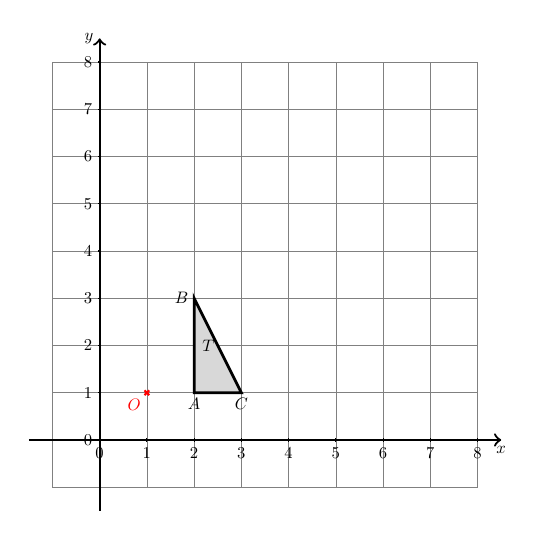
\begin{tikzpicture}[scale=0.6, transform shape]
    \def\axisLimit{8}

    \definecolor{borderColour}{HTML}{000000}
    \definecolor{fillColour}{HTML}{D8D8D8}

    % Draw grid
    \draw[step=1cm,gray,very thin] (-1,-1) grid (\axisLimit,\axisLimit);

    % Draw axes
    \draw[thick,->] (-1.5,0) -- (\axisLimit+0.5,0) node[anchor=north] {$x$};
    \draw[thick,->] (0,-1.5) -- (0,\axisLimit+0.5) node[anchor=east] {$y$};

    % Label x-axis and y-axis
    \foreach \x in {0,1,...,\axisLimit}
        \draw (\x cm,1pt) -- (\x cm,-1pt) node[anchor=north] {$\x$};
    \foreach \y in {0,1,...,\axisLimit}
        \draw (1pt,\y cm) -- (-1pt,\y cm) node[anchor=east] {$\y$};

    % Centre of enlargement
    \coordinate (COE) at (1,1);
    \draw[red, thick] (COE) node[below left] {$O$};
    \draw[red, thick, mark=x] plot coordinates {(1,1)};

    % Original triangle T
    \coordinate (A) at (2,1);
    \coordinate (B) at (2,3);
    \coordinate (C) at (3,1);

    \draw[fill=fillColour, draw=borderColour, line width=1pt] (A) -- (B) -- (C) -- cycle;
    \node at (2.3,2) {$T$};
    \node[below] at (A) {$A$};
    \node[left] at (B) {$B$};
    \node[below] at (C) {$C$};

\end{tikzpicture}
\end{center}

\noindent Triangle $T$ has vertices $A(2,1)$, $B(2,3)$ and $C(3,1)$.

\noindent Find the coordinates of the vertices of the image of triangle $T$ after an enlargement with scale factor $2$, centre $O(1,1)$.

\vspace{4cm}
\begin{flushright}
    \answerplain{2}
\end{flushright}
\end{question}